\subsection{Compass Implementation}
The PmodNAV was connected to the ZedBoard via one of its Pmod connectors. The PmodNAV was controlled by a Pmod connected to the ARM Processor of the SoC so that the compass data was able to be directly combined with the rangefinder's data before it was written to the FPGA. However, only one of the ZedBoard's five Pmod connectors is directly connected to the ARM Processor, and it was already used for communication with the rangefinder. One Pmod connected to the FPGA fabric was re-routed to be controlled by the ARM Processor through capability provided by the Zynq7 Processing System.

\subsubsection{Re-Customizing the Zynq7 Processing System}
The Zynq7 Processing System was easily re-customized to account for the PmodNAV's specifications. SPI functionality was added in the processing system's customization window under I/O Peripherals in the MIO Configuration tab. The SPI pins were routed to Extended MIO (EMIO) to allow one of the ZedBoard's FPGA-controlled Pmods to be controlled by the ARM Processor. Since both SPI0 and SPI1 support EMIO capability, SPI0 was arbitrarily chosen over SPI1. This process is shown in Figure \ref{enabling_spi0}.

\begin{figure}[H]
	\centerline{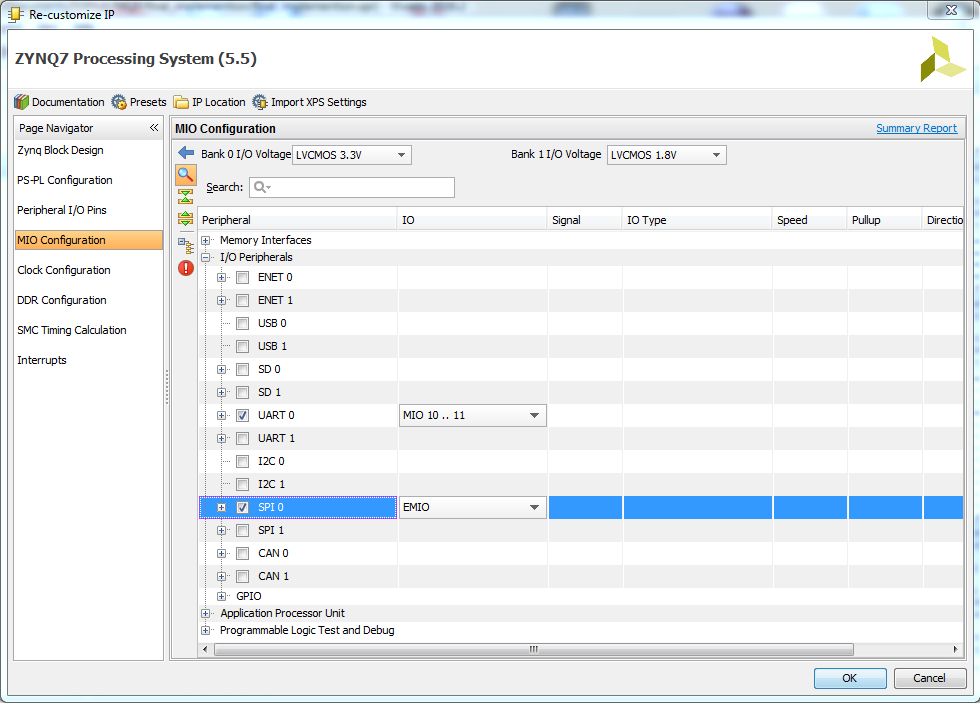
\includegraphics[width=1\textwidth]{enabling_spi0.png}}
	\caption{Re-Customizing the Zynq7 Processing System to Add SPI}
	\label{enabling_spi0}
\end{figure}





